\part{Results}
\label{part:results}

\chapter{Results}

For the following reslts, I ran 230 simulations per ratchet, we calculate the mean angular velocity over the different seeds for each frequencies between 0Hz and 10Hz, and to validate the accuracy of each result, we used the error over the mean~\cite{altman2005standard}:

\begin{equation}
  \sigma_{\bar{x}} = \displaystyle\frac{\sigma}{\sqrt{n}}.
  \label{eq:errormean}
\end{equation}

Figure~\ref{fig:angularvsfrequency} summarizes the main result of this work, showing how the average angular velocity of the system changes with the frequency of the rotating magnetic field. At low frequencies (0–3 Hz), the internal dipoles of the paramagnetic colloids can align and rotate in phase with the external field, producing almost no net rotation on the solid ratchet. In this regime, particles are merely diffusive and are stuck in a crystaline structure, which aligns with theoretical expectations.
As the frequency increases, the dipoles begin to experience a delay relative to the field rotation. This phase lag reduces the alignment efficiency, and the system gradually loses synchronization, reaching a peak mean angular velocity at 5 Hz. Beyond this critical frequency, the particles no longer move by exchanging neighbors but instead start to experience an repulstion and attraction force between each pair of particles, mimicking the behavior of an harmonic bond.
At the same time we observe that the geometry of the ratchet does not play a significant role in the speed; however, it has a non-negligible impact for the spin down ratchets.
This demonstrates how the balance between magnetic coupling and field rotation controls the system's dynamics. 
%%%%

\begin{figure}[h]
\begin{center}
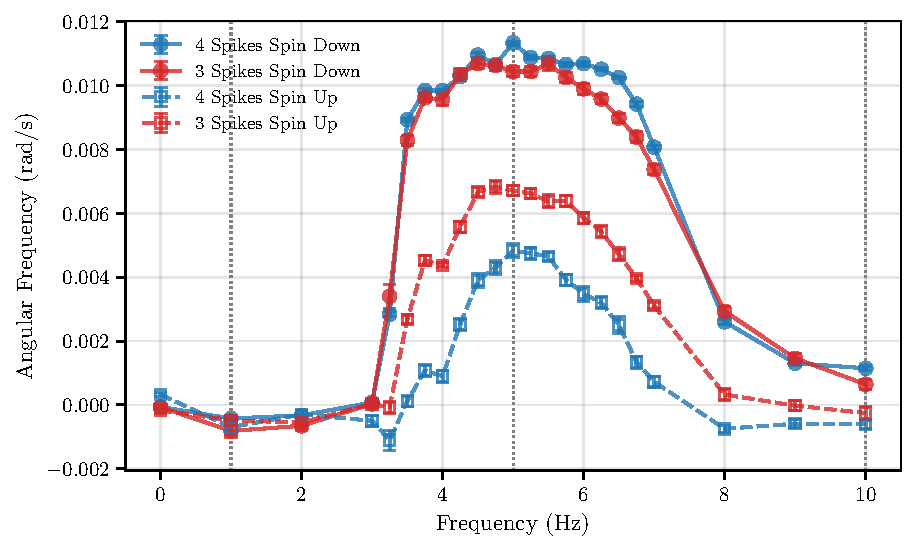
\includegraphics[width=0.95\textwidth]{figures/AvsF.pdf}
\end{center}
\caption[Angular velocity as a function of driving frequency.]
{Average angular velocity of the paramagnetic colloidal cluster as a function of the rotating magnetic field frequency. Vertical guides at 1, 5, and 10 Hz highlight specific frequency values.}
\label{fig:angularvsfrequency}
\end{figure}


Figure~\ref{fig:particletrj} shows the particle trajectories for three representative cases: 1 Hz, 5 Hz, and 10 Hz. When no field rotation is applied (0 Hz), the particles move randomly due to thermal noise, producing isotropic diffusion with no net direction, nonetheless at a frequency of 1 Hz, the particles' magnetic moment rotates at the same speed as the magnetic field creating rotation with pairs, but staying almost fixed in the same place. At 5 Hz, however, their trajectories reveal a ballistic pattern, indicating that the dipoles are not synchronized with the external field and move collectively. This difference confirms that the rotation frequency of the magnetic field directly controls the transition from random to directed motion, as also reflected in the angular velocity results shown in Fig.~\ref{fig:angularvsfrequency}, I highlighted the trajectory of one single particle to be able to see the difference in the behavior they show for each driving frequency. For 1 Hz, the trajectory show the rotation tendency they form each pair of particles, however they do not move far from their shared center of mass, nevertheless for 5 Hz it is evident the chaotic movement the particles have, and finally for 10 Hz the particles seem to be quasi-static.

\begin{figure}[h]
\begin{center}
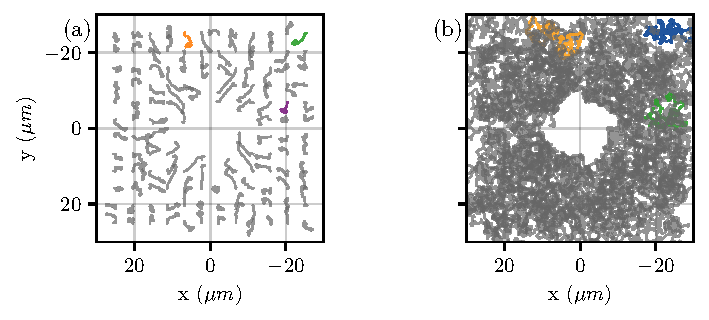
\includegraphics[width=0.95\textwidth]{figures/parttrj.pdf}
\end{center}
\caption[Particle trajectories at different driving frequencies.]
{Trajectories of the particles of one simulation during the simulation, from 50 - 100 s, for (a) 1 Hz, (b) 5 Hz, and (c) 10 Hz. The highlighted trajectories are the same particles.}
\label{fig:particletrj}
\end{figure}

Since the angular velocity has very strong fluctuations, a graph over the time will not give us important visual guides wether to determine the properties. Therefore we used a type of convolution known as moving average to obtain a smoother plot. This type of mean focus on a group of values to then forget them to focus on another new group. According to ~\cite{hyndman2025moving} a two and one sided averges are given respectively by Eq. (\ref{eq:movingaverage}), which is, in fact, a low-pass filter, perfect for the large fluctuations.

\begin{align}
  z_t &= \frac{1}{2k+1} \sum^{k}_{j =-k} y_{t+j}, \quad t=k+1, k+2,\dots,n-k,\\
  z_t &= \frac{1}{k+1} \sum^{k}_{j =0} y_{t-j}, \quad t=k+1, k+2,\dots,n.
  \label{eq:movingaverage}
\end{align}

Figure~\ref{fig:velocityvstime} presents the time evolution of the angular velocity. At 0 Hz, the system exhibits only random fluctuations caused by thermal noise, with an average angular velocity close to zero. In contrast, at 5 Hz, the angular velocity remains consistently positive over time, despite instantaneous fluctuations. The rolling mean highlights this difference, showing a net rotational trend, in certain points, that reflects the impact the collective rotation of colloids have in the rotation of the ratchet.

\begin{figure}[h!]
\begin{center}
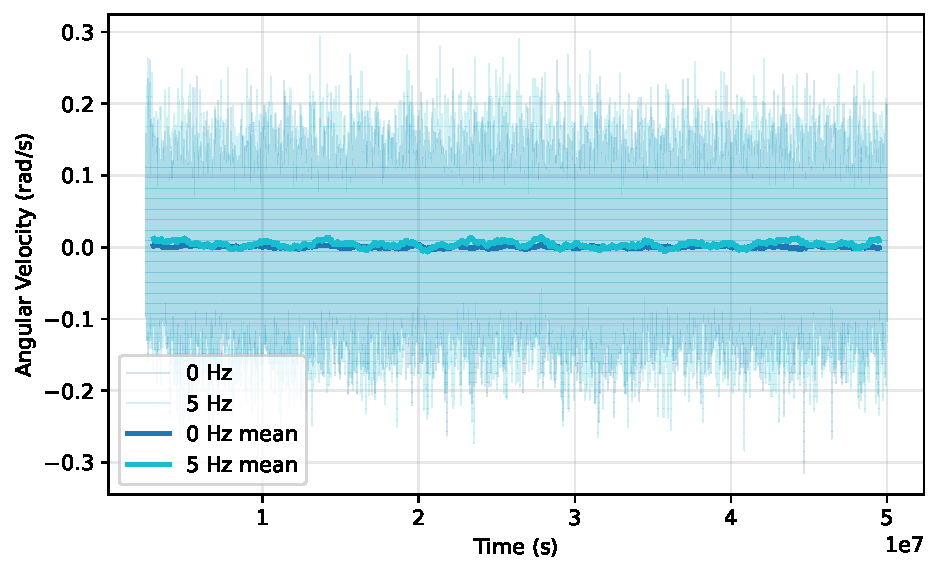
\includegraphics[width=0.95\textwidth]{figures/time_series.pdf}
\end{center}
\caption[Angular velocity as a function of time.]
{Angular velocity of the ratchet as a function of time for a single simulation at 1 Hz and 5 Hz. The shaded regions correspond to the raw data, and the solid lines show the rolling mean.}
\label{fig:velocityvstime}
\end{figure}

Due to the inherent variability of stochastic processes, a large amount of data is required to obtain reliable statistics. Figure~\ref{fig:histogram} shows the angular velocity histograms for 0 Hz and 5 Hz. Interestingly enough, the data showed a gaussian distribtuion and to better visualize the shape of the graph, we used a Gaussian Kernel Density Estimation (KDE) to smooth out the histogram ~\cite{chen2017tutorial}. 

\begin{equation}
  \hat{p}_n = \frac{1}{nh^d} \displaystyle\sum_{i=1}^{n}K \left(\frac{x - X_i}{h}\right)
  \label{eq:kde}
\end{equation}

\begin{equation}
  K(x) = \frac{exp(-\abs{\abs{x}}^2/2)}{v_{1,2}}, \quad v_{1,2} = \displaystyle\int exp(-\abs{\abs{x}}^2/2)dx.
  \label{eq:gaussiankernel}
\end{equation}

At 1 Hz, the mean lies almost exactly at 0 rad/s, while the 5 Hz distribution is skewed to the left, indicating a high probability of a positive net rotation and backing up the results of Figure~\ref{fig:velocityvstime}. 


\begin{figure}[h!]
  \begin{center}
    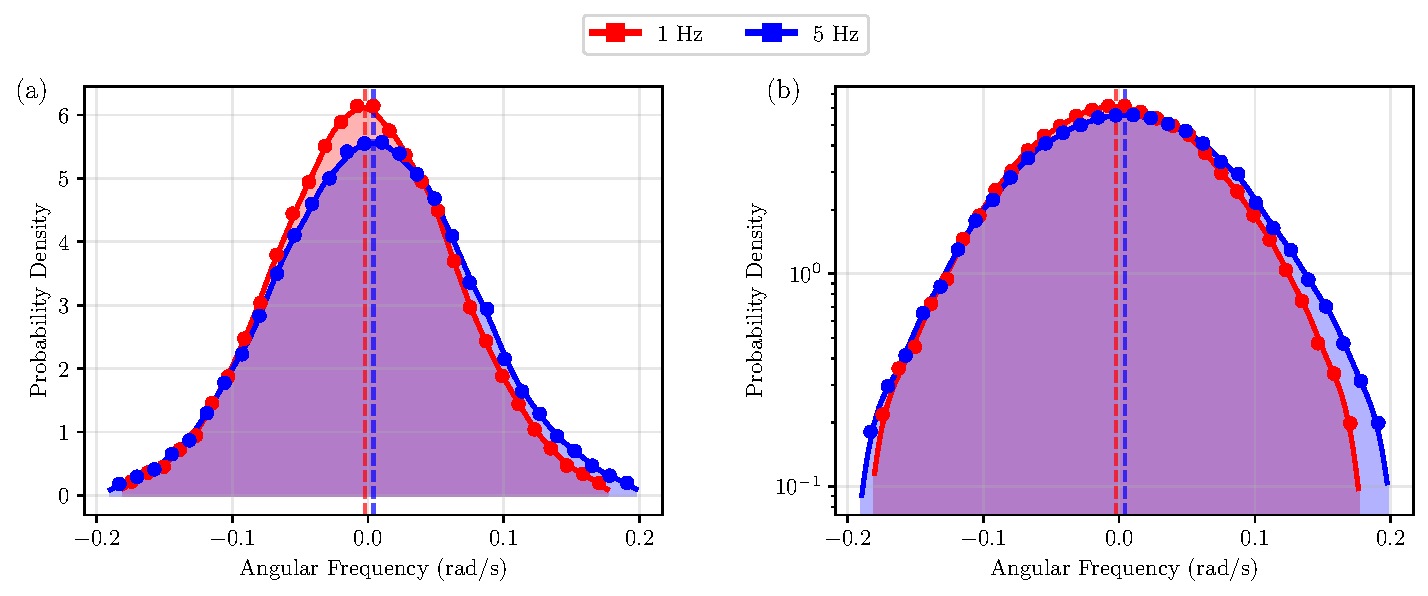
\includegraphics[width=0.95\textwidth]{figures/histogram_comparison.pdf}
  \end{center}
  \caption[Histogram of angular velocity.]{\textbf{Panel a)} Histogram of angular velocity of the ratchet for a single simulation at 1 Hz and 5 Hz. \textbf{Panel b)} Histogram with semilogaritmic scaling.}\label{fig:histogram}
\end{figure}

The angular velocity is extremely small, however Figure~\ref{fig:particleangulardisplacement} shows the angular displacement of a single ratchet particle over the entire simulation. At 1 Hz, the particle shows an initial displacement but remains largely constant over time, experiencing only thermal fluctuations. This initial displacement can be due the initial interaction of the closer colloids, which move close to the walls of the ratchet and probably moving or rotating the ratchet a certain, but negligible amount, however, the remarking section is the tendency of not moving for a long period of time. In contrast, at 5 Hz, the particle exhibits a net displacement that appears linear in time, clearly showing a non zero velocity.

To give meaning to the plot, we can obtain the arc length of a circle, this is assuming this as an ideal trajectory for the ratchet, therefore we use the following equation:

\begin{equation}
  s = r\theta,
  \label{eq:arclength}
\end{equation}

where $s$ is the arc length, r is the radius of our ratchet and $\theta$ is the angle formed from the particle to the initial position.
In this case we can see that its final angular position is $\theta \approx 2 rad$, which corresponds to the total distance traveled by the particle was $s \approx 16 \mu m$.

In the total simulation, the ratchet experienced a little less than half rotation but more than a quarter, but according to Purcell~\cite{purcell2014life}, at those regimes movement not necessarily has to be much. Nevertheless, this provides clear evidence of the frequency's dramatic effect on ratchet rotation. This aligns with the theoretical principle that work cannot be extracted from thermal fluctuations alone. However, we have identified a range of frequencies where colloidal interactions and a driving magnetic field are sufficient to drive ratchet rotation.


\begin{figure}
  \begin{center}
    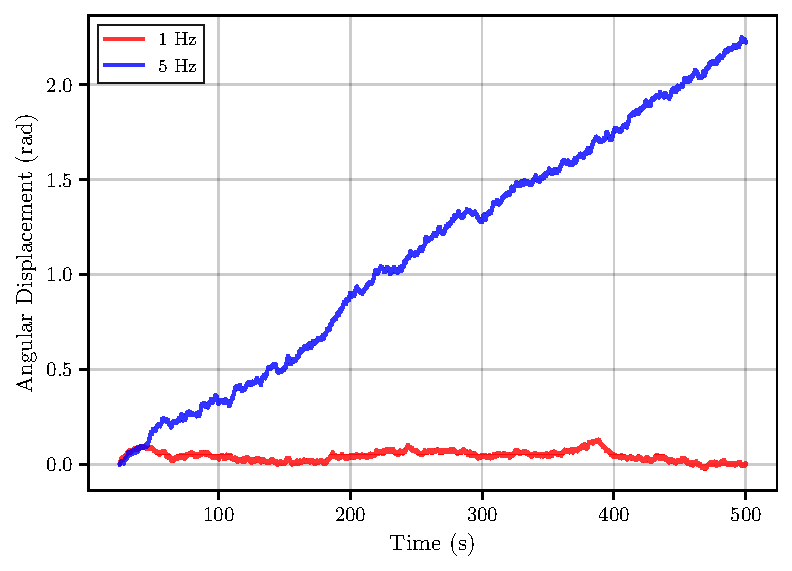
\includegraphics[width=0.95\textwidth]{figures/particle_displacement.pdf}
  \end{center}
  \caption[Angular displacement of a particle.]{Angular displacement of a particle of one simulation at 0 Hz and 5 Hz.}\label{fig:particleangulardisplacement}
\end{figure}

